\documentclass[10pt]{article}
\usepackage{graphicx}
\usepackage[margin=3cm]{geometry}
\usepackage[usenames,dvipsnames]{color}
\usepackage{array}
\usepackage[colorlinks=true, urlcolor=MidnightBlue]{hyperref}
\usepackage{fancyhdr}
\usepackage{fixltx2e} % \textsubscript
\usepackage{layout}

%%% Measurements %%%
% \topmargin=-0.3in
\oddsidemargin=0in
\evensidemargin=0in
\textwidth=6.5in
\marginparwidth=0.5in
% \headheight=0pt
\headsep=0pt
\textheight=670pt

%%% Table formatting %%%
\definecolor{lightgray}{gray}{0.8}
\newcolumntype{L}{>{\raggedleft}p{0.14\textwidth}}
\newcolumntype{R}{p{0.8\textwidth}}
\newcommand\VRule{\color{lightgray}\vrule width 0.5pt}

\title{JAMIE A. MACDONALD}
\author{\href{mailto:jamie.alban@gmail.com}{jamie.alban@gmail.com}\\(613) 583-7654\\2251 Fife Cres.\\Ottawa, ON}
\date{}

\renewcommand{\headrulewidth}{0pt} % no rule for header

\lfoot{\href{https://twitter.com/JamieMacdo}{@JamieMacdo}}
\cfoot{\href{https://github.com/jameh}{github.com/jameh}}
\rfoot{\href{https://ca.linkedin.com/in/jamiemacdo/}{ca.linkedin.com/in/jamiemacdo/}}

\begin{document}
%%% Center Name and email %%%
\begin{minipage}{0.2\textwidth}
\hspace{0em}
\end{minipage}
%%% Name and email %%%
\begin{minipage}{0.55\textwidth}
\vspace{-3em}
\maketitle
\end{minipage}
%%% Picture %%%
\begin{minipage}{0.25\textwidth}
\flushright{
    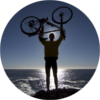
\includegraphics
    {jamie_alban_small.png}
}
\end{minipage}
\thispagestyle{fancy}
\vspace{-3em}
\section*{Objective}
I am looking for immediate fulltime service- or sales-oriented employment. I have a deep desire to give back to the community which supported me in my four-year engineering undergrad at Queen's. I enjoy sparking relationships with strangers and am a devoted worker. Furthermore, I have a strong mathematics and programming background, and always strive to solve real-world optimization problems.
\vspace{-1em}
\section*{Education}
\begin{tabular}{L!{\VRule}R}
2010--2014&{\bf BSc Mathematics \& Engineering, Computer and Communication Systems}\\
          &{Queen's University, Kingston Ontario}\\
\end{tabular}
\vspace{-1em}
\section*{Projects}
\begin{tabular}{L!{\VRule}R}
2013--2014&{\bf Channel-Optimized Vector Quantization of Correlated Images for Transmission over a Wireless Channel (Fourth Year Project/Thesis)}\\
          &{Design \& implement a Lossy Joint Source-Channel Code which exploits the Correlation in two random sources (images)}\\
          &{(Information Theory, Discrete Cosine Transform, C programming, Python matplotlib, LaTeX writeup)}\\
2010&{\bf Child Soldier Cycle (Activism)}\\
    &{Biked 3000km from Ottawa to Newfoundland running an awareness campaign for child soldiering -- collected over 1500 red handprints as a petition to the media to provide better coverage of global Child Soldiering issues}\\
    &{Leadership, outreach, perseverance, organization}\\
\end{tabular}

\vspace{-1em}
\section*{Work Experience}
\begin{tabular}{L!{\VRule}R}
  2009&{\bf Customer Service Rep. / Registration -- Canterbury Pool, City of Ottawa}\\
        &{Cash transactions; Course registration; Public relations for instructors}\\
  2009-2010&{\bf PT Lifeguard/Swim Instructor -- Canterbury Pool, City of Ottawa}\\
  Summer 2011&{\bf Park Programmer -- Canterbury Park, City of Ottawa}\\
        &{Entertain and supervise children at wading pool}\\
        &{Standard First Aid, National Lifeguard Service, AED \& Oxygen, Swim Instructor}\\
	Summer 2014&{\bf Software Programmer -- IBM Watson Visualization Engine}\\
			  &{Maintain charting/vis engine (Java); frontend JS demo app; agile development; Java AWT, canvas; GeoJSON}\\
			  &{Collaborate with an international team; build strong communication skills}\\
\end{tabular}

\vspace{-1em}
\section*{Activities}
\textbf{Clubs}: Queen's Hack Nights\\
\textbf{Programming}: Web app development\\
\textbf{Recreation}: Yoga, Biking, Longboarding\\
\textbf{Music}: Keys, Trumpet, Voice (let's jam!)

\end{document}
